
\documentclass[12pt]{article}
\usepackage{geometry}
\usepackage{amsmath,bm}
\usepackage{sectsty}
\usepackage{graphicx}
\usepackage{tabularx}
\usepackage{hyperref}
\usepackage{amsfonts}
\usepackage{url}
\setlength{\parskip}{1em}
\setlength{\parindent}{0 pt}
\usepackage[font=small,labelfont=bf]{caption}
%\numberwithin{equation}

\begin{document}
    \title{Model independent measurement of production of two jets with two charged lepton pairs in Large Hadron Collidor at ${\sqrt{\text{s}} = 13\ \text{TeV}}$}
    \author{Qichen Dong}
    \maketitle

    \begin{abstract}
        This report 
    \end{abstract}
    \newpage

    \section{Introduction}
        \par Vector boson scattering (VBS) process is important as a pure electroweak interaction to 
        probe the nature of electroweak symmetry breaking (EWSB). At the TeV scale, VBS process alone violated the longitudinally
        unitarity, however, in the standard model (SM), the apparence of higgs boson cancels the violation rigorously. Since higher order effects 
        beyond the SM (BSM) are suppressed tromendusly at low energy scale, study of VBS process in higher energy scale may gives hints of BSM theories 
        which offer alternative EWSB machenisms to break the elegent cancellation of longitudinally unitarity. Moreover, study of the VBS process provides
        a good chance to observe the CP violating effects that contribute to the large matter antimatter asymetry observed in the universe. Since no CP 
        vioaltion effect is predicted in the SM in the VBS process, only sources of CP violation come from BSM theories which interfere with the SM. 

        \par \noindent In the Large hardron collidor (LHC), VBS events are produced by a pair of vector bosons which produced by initial partrons scattered into another
        pair of vector bosons. At detector level, events with two jets associated with 2 pairs of leptons originated from vector bosons pair are the signiture of
        VBS process. Despite the complexity of final states, background processes other than the VBS can also produce exactly the same final state particles, we
        denote these processes $jjVV$, one of the main $jjVV$ background is $jjVV$ production with strongly interacting verteices ($S\ jjVV$). The most VBS concentrated 
        channel is $jjVV$ processes with only electroweak verteices, denote as ($EW\ jjVV$). Figure 1 shows example Feynman diagrams of leading order $S\ jjZZ$ and $EW\ jjZZ$ processes\cite{ATLAS-CONF-2019-033}.
        \begin{figure}[ht]
            \begin{centering}
            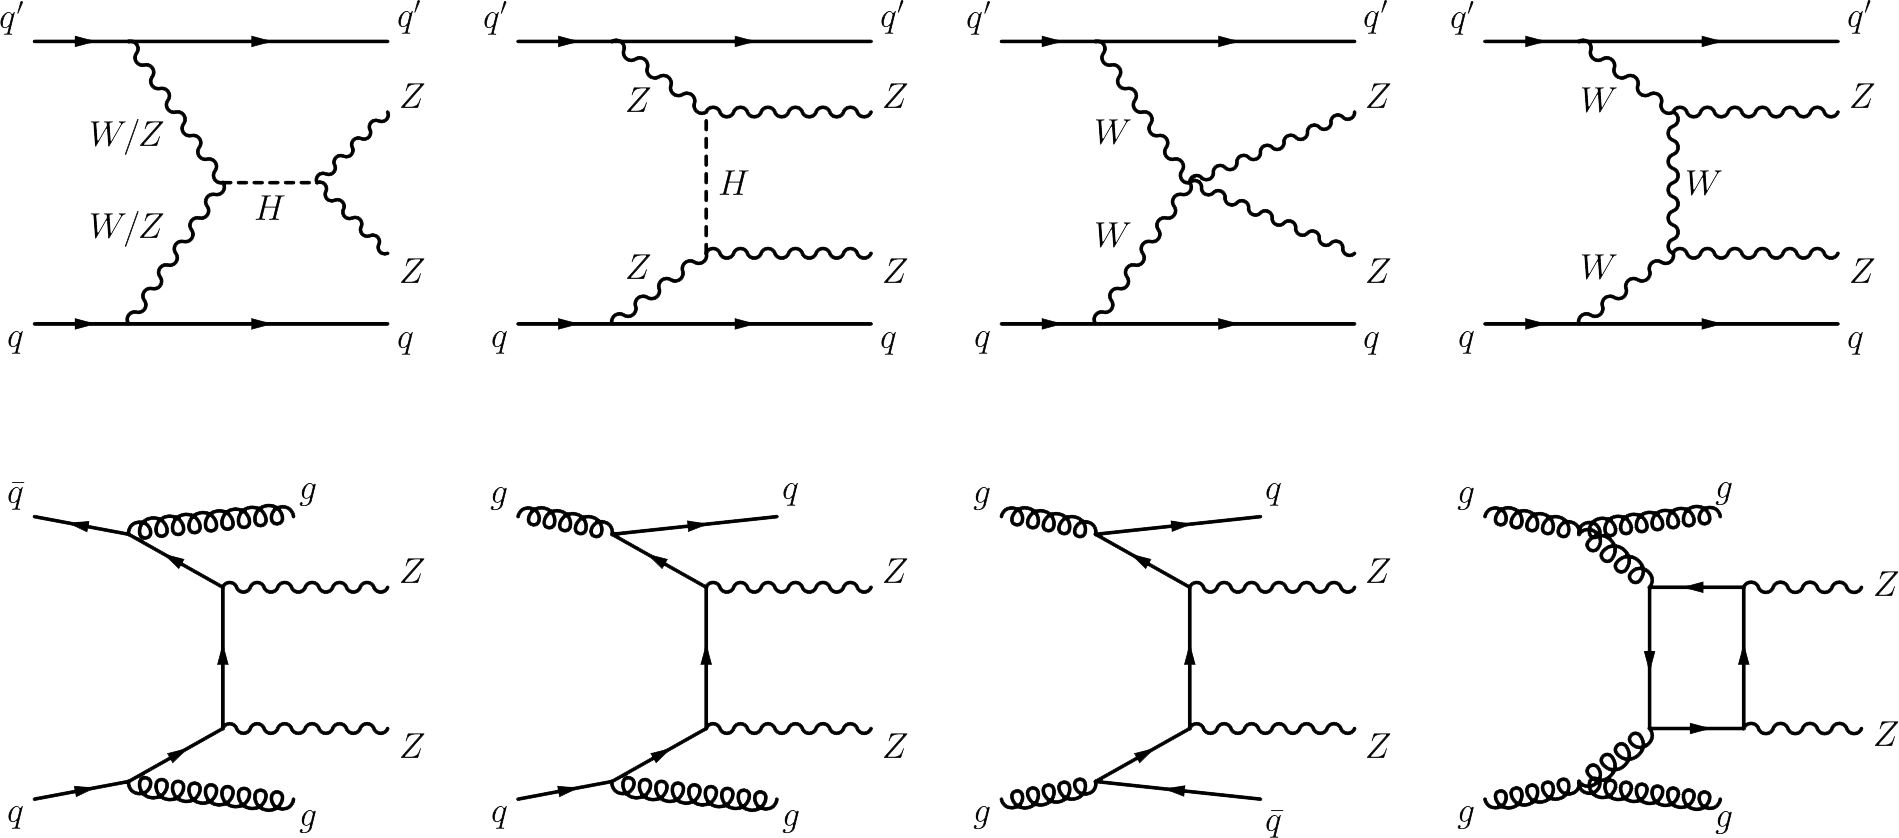
\includegraphics[scale=0.42]{Feynman_diag.png}
            \caption{The first order feynman diagrams contributing to $jjZZ$ processes, the first line is $EW\ jjZZ$ and the second line is $S\ jjZZ$ processes.}
            \end{centering}
        \end{figure}
        \par Despite same final state particle in leading order $EW\ jjVV$ and $S\ jjVV$ process, the geometry configuration of them are quite different, 
        Electroweak jjVV production process is expected to have a much larger jets separation since two heavy vector bosons emitted from each of the initial state 
        quarks, while the Strong jjVV production is expected to be more likely to radiate additional jets since quark and gluon carrys color charge. Moreover, the vector
        bosons  produced by EW jjZZ process are more centralised between the two associated jets and more balanced in $p_T$. These informations were used to define the
        signal region and control regions in the measurement.
        \par The $EW\ jjVV$ process in which both vector bosons decay leptonically is extremely rare with cross section around $1fb$ in current energy scale, but it is a relatively 
        clean channel with minimal hardronic background. In this report, only events with final states contain 2 pairs of charged leptons from Z bosons was considered as signal, denote as $jjZZ4l$,
        other procedures were considered as backgrounds.

        \par In this report, the $36 fb^{-1}$ pp collision data with centre of mass energy $\sqrt{s} = 13 TeV$ collected by the atlas detector 
        in 2016 is used, the differential cross section of VBS process and irreduceable background in a VBS enhanced fidutial phase space is measured.
        The experimental effect induced by the detector is removed by unfolding with the help of simulation events, so that the results can be directly 
        compared by future \nopagebreak experiments.

    \section{ATLAS detector}
        \par The performance and geometry detail of ATLAS detector can be found in reference\cite{Collaboration_2008}.
        ATLAS detector is a general-purpose layered-design particle detector built in 2008, which is cylindrically symmetric to the beam axis with near complete coverage in solid angle.
        The first layer, inner tracking detector covering pseudorapidity range $|\eta| < 2.5$ is submerged in 2T axial magnetic field produced by superconducting electromagnet, which is designed to track charged particles. 
        The second layer is the complex of electromagnetic calorimeter and hardroninc calorimeter, where particles interact with the material and deposit energy, both covering $|\eta| < 3.2$. In the region where $4.9> |\eta| > 3.2$, 
        a forward electromagnetic and hadronic calorimeters is used.
        The third layer is the large muon spectrometer covering $|\eta| < 2.7$, due to the high penetrating power of muon, both calorimeter cannot 
        stop muons, much larger apperatus is used to capture their track.
        Around 25 $pp$ collides (2016) in the center of the detector each time beams cross the detector, 
        resulting around 1 billion collisions per second, most of which are elastic collision contain little information, 
        complicate hardware and software online trigger system\cite{Nedden_2017} is 
        used to cutdown events rate to about 1000 per second for analyists to study offline. 
        A cut-away view of the ATLAS detector with main components labeled is shown in Figure 1\cite{Collaboration_2008}.
        \begin{figure}[ht]
            \begin{centering}
            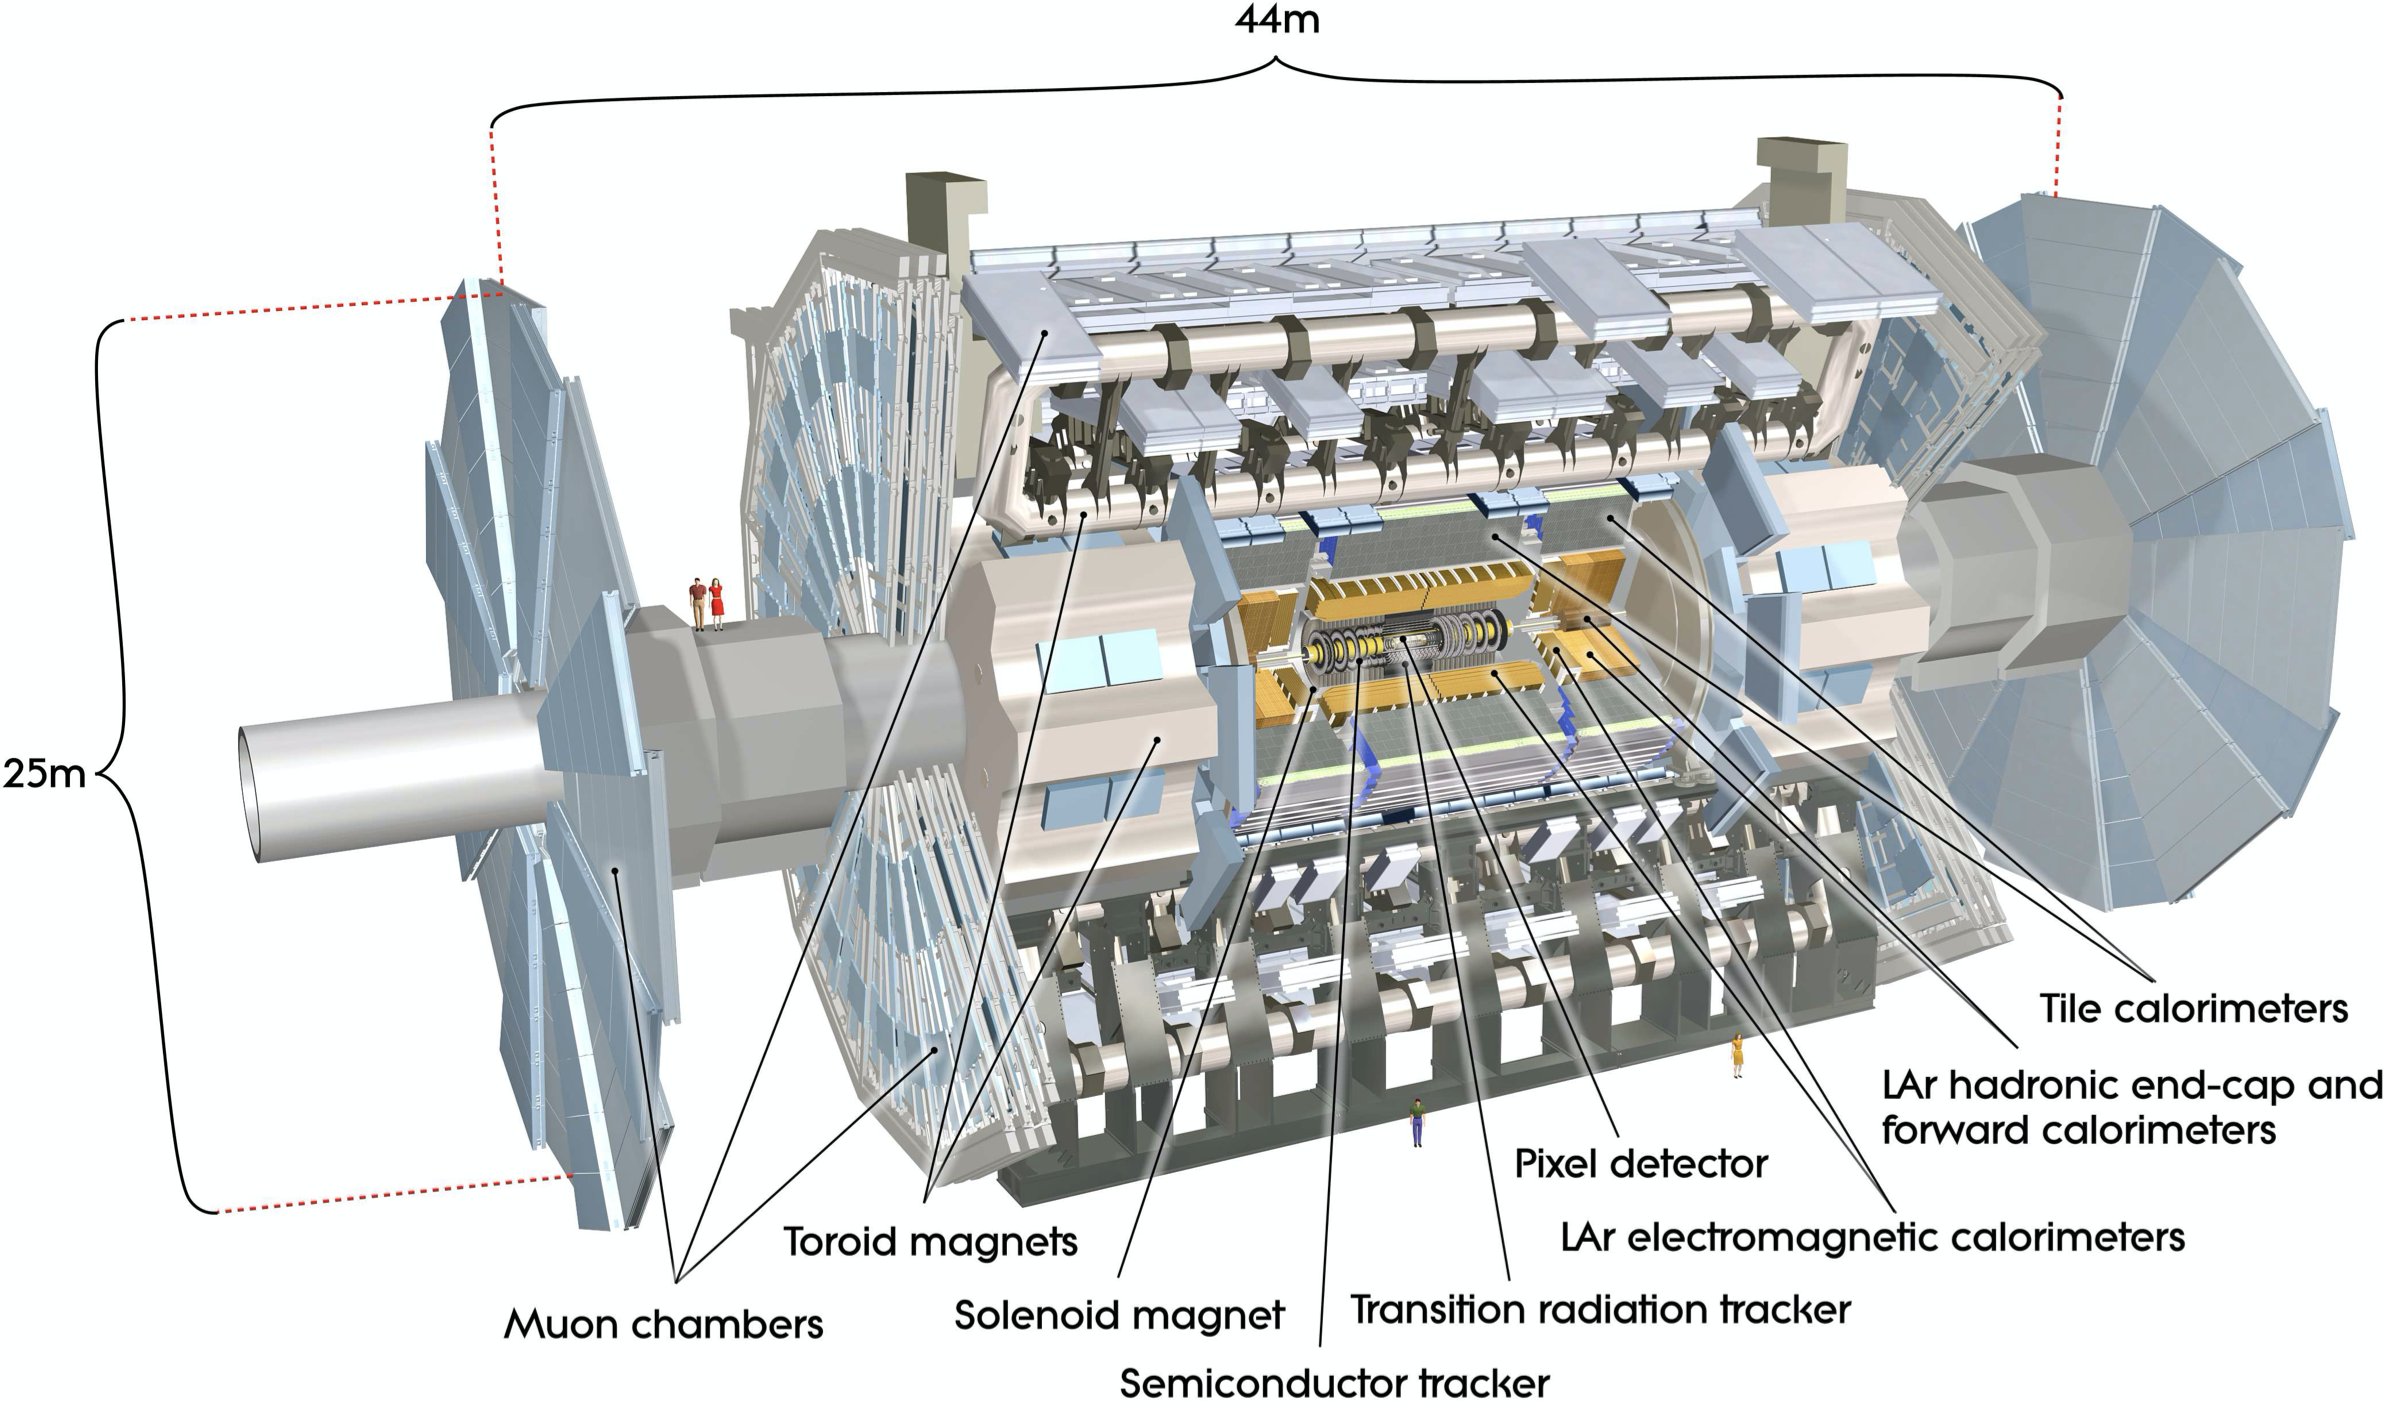
\includegraphics[scale=0.35]{atlas_det.png}
            \caption{A cut-away wiew of the ATLAS detector, major components and the dimension of it is labeled.}
            \end{centering}
        \end{figure}
    \section{Data and Simulation}
        \par The measurement is performed using the pp collision data recorded during 2015 and 2016 run of LHC with $\sqrt{s} = 13\ TeV$.
        During this peroid, an integrated luminosity of $36fb^{-1}$ is obtained. Data taken in 2017 and 2018 run can be used in 
        the future for further analysis.
        \par Simulation for various processes used in the measurement are generated by different Monte Carlo (MC) generators, three generations 
        of simulation events corresponding to 3 years of LHC run with different pile up and integrated luminosity are available, adding up 
        to simulation data corresponding to a total of $139fb^{-1}$. Only the simulation data corresponding to 2015-2016 run was used in this measurement
        to have best prediction to the data.
        The $EW jjZZ$ process is modeled by Sherpa2.2.2\cite{0811.4622} with NNPDF3.0NNLO\cite{1405.0301} partron distribution function (PDF) at leading order (LO).
        The vector boson fusion (VBF) higgs contribution is modeled using POWHEGVBF\_H\cite{0911.5299} configuration with Pythia8\cite{1410.3012} showering and NNPDF3.0 PDF.

        The $S\ qq \rightarrow jjZZ$ process is generated by Sherpa2.2.2 with NNPDF30NNLO PDF, events with less then 2 jets are generated at next to LO(NLO), others are generated 
        at LO, while $t\bar{t}\rightarrow {H} \rightarrow ZZ$ contribution is generated separately by POWHEG\cite{1007.3893} with Pythia8 showering and NNPDF2.3 PDF.
        The $S\ gg \rightarrow jjZZ$ process is modeled using Sherpa2.2.2 with NNPDF30NNLO PDF, again, the $gg\rightarrow {H}\rightarrow ZZ$ is modeled separately with POWHEG and Pythia8.

        \par The production of $jjWZ$ events is produced by POWHEG with Pythia8. The EW triboson process with the same order of $\alpha=6$ is modeled by Sherpa2.2.2 with NNPDF30NNLO PDF.
        Single Z boson decay is modeled by Sherpa with NNPDF30NNLO PDF while $t\bar{t}Z$ decay is modeled separately with the same configuration. $t\bar{t}$ production is modeled by 
        POWHEG with Pythia8 showering.

        \par All simulations were include detailed detector simulation by Geant4\cite{AGOSTINELLI2003250}.  
        both simulated events and the data were reconstructed using raw spatial and momentum of leptons and 
        jets in CERN ROOT\cite{ANTCHEVA20092499} framework.

    \section{Candidates selection}
        \par selecting the desired $ZZ4l$ events while substracting other background effects 
        is challenging, while distinguishing $EW jjZZ$ and $S jjZZ$ is even harder, the 
        final states of both process are identical but we can still study the differences
        in geometry information and possible associated process of these events. The selection used in 
        this report is largly similar to the selection detailed in ref. \cite{ATLAS-CONF-2019-033}.
        \par The detector level selection relies on the properties of all final state particles, namely charged leptons
        and jets. 
        \par Jets within $|\eta| < 2.4$ were required to have transverse momentum ($p_{T}$) higher than 30 GeV,
        jets with higher pseudorapidity $2.4 < |\eta| < 4.5$ must have $p_T > 40$ GeV. 
        \par Muons were identified by compatible tracks in the muon spectrometer and the inner tracking detector. 
        outside the region of inner tracking detector, muons can also be identified by an MS track alone. 
        The identified muons described above are required to have $p_{T} > 7 $GeV. Muons are required to have $|\eta| < 2.7$  and satisfy
        ``loose'' particle identification criterion. Electrons were identified using the information of the EM calorimeter and 
        corresponding tracks in the inner tracking detector. Electrons is also required to satisfy ``loose'' identification working point, 
        and have $p_{T} > 7 $GeV and $|\eta| < 2.47$.
        \par A ``FixedCutPflowLoose" lepton isolation creteria\cite{Aaboud_2019} is required by all identified charged leptons to 
        remove leptons overlap with jets. Furthermore, the tracks of leptons were required to have transverse impact parameter $d_0$ and 
        longitudinal impact parameter $z_0$ satisfying $d_0/\sigma_{d_0} < \text{5}$ and $z_0\text{sin}\theta < 0.5 \text{\ mm}$.
        \par \emph{TODO::OVERLAP REMOVAL}

        \par the resonance of Z boson pair were recostructed by two pairs of same flavor, opposite charge (denote SFOC) leptons passed 
        detector level selection, the tracks of two SFOC lepton pairs are required have separation $\Delta R > 0.2$, 
        where $\Delta R = \sqrt{{\Delta\eta}^2 + {\Delta\phi}^2}$, moreover, the three leading leptons with higher $p_T$ are required to have 
        $p_T > 20, 20, 10$ respectively. if more then two candidate OSFC lepton pairs were avilable, the lepton pairs with invarient mass($m_{l^+l^-}$) closest 
        to Z boson mass were selected. the lepton pair with mass closest to Z boson mass are required to have invarient mass $70GeV < m_{Z_1} < 110GeV$ and the 
        other have $21\ GeV < m_{Z_1} < 110GeV$.
        \par Events must have at least two jets pass detector level selection, the leading and subleading jets with $y_{j_1} \times y_{j_2} < 0$ and $|y_{j_1} - y_{j_2}| > 2$
        and dijet invarient mass $m_{jj} > 200 GeV$ and $P_{Tj_1} > P_{Tj_2}> 30 GeV$ were selected. 
        \par The $EW jjZZ$ events are predicted to be more balanced in $P_T$, which is parametrised by 
        $$P_{T\ balance} = |\frac{P_{T\ jjZZ}}{P_{T\ Z_1} +  P_{T\ Z_2} +  P_{T\ j_1} +  P_{T\ j_2}}|$$
        where $P_{T\ jjZZ}$ is the total $P_T$ of the 4 leptons 2 jets system and the denominator is the scalar sum of individual $P_T$.

        \par With the fiducial phase space defined, signal region (SR) and control regions (CR) are further defined base on centrarity and
        the apperence of additional jets inbetween (denote $nIBj$) the leading and subleading jets. The centrarity is defined as
        $$C_{ZZ} = \frac{y_{jj} - y_{ZZ}}{y_{j_1}-{y_{j_2}}}$$
        which indicates how the Z boson pair system is centraised in the dijet system. In SR region, events are required to have $C < 0.5$ 
        and $nIBj=0$, outside of which were defined as conjagate CR. Table 1 summarise the SR and CR definition used in the analysis. 
        \begin{table}[ht]
            \centering
            \renewcommand\arraystretch{1.2}
            \begin{tabularx}{\textwidth}{X c} 
            \hline\hline
            Objects &  \begin{tabular}{p{2cm}  p{2cm}  p{2cm}  p{2cm}} SR & $\text{CR}_{C_{ZZ}}$ & $\text{CR}_{jIB}$ & $\text{CR}_{all}$ \end{tabular}\\ 
            \hline\hline
            Electrons & \begin{tabular}{c} ``Loose'' ID criterion\\ ``FixedCutPflowLoose'' criterion\\$p_T > 7 \text{\ GeV},\ |\eta| < 2.47$ \\ $|d_0/\sigma_{d_0}| < 5,\  |z_0 × \text{sin}\theta| < 0.5 \text{mm}$\end{tabular} \\
            \hline
            Muons & \begin{tabular}{c} ``Loose'' ID criterion\\ ``FixedCutPflowLoose'' criterion\\$p_T > 7 \text{\ GeV},\ |\eta| < 2.7$ \\ $|d_0/\sigma_{d_0}| < 3,\  |z_0 × \text{sin}\theta| < 0.5 \text{mm}$\end{tabular} \\
            \hline
            Jets &  $P_T > 30(40) \text{GeV}$ for $|\eta| < 2.4(2.4<|\eta| < 4.5)$ \\
            \hline
            OSFC lepton pairs & \begin{tabular}{c} two pairs of OSFC lepton with $M_Z$ closest to Z mass \\ $p_T > 20, 20, 10$ GeV for leading 3 leptons \\ $\Delta{R_{l^+l^-}} > 0.2$ \\$70\ \text{GeV}<M_{Z_1} < 110$ GeV \\ $21\ \text{GeV}<M_{Z_2} < 110$ GeV\end{tabular} \\
            \hline
            Dijets system & \begin{tabular}{c}leading two jets with $y_{j_1} \times y_{j_2} < 0$ and $|y_{j_1} - y_{j_2}| > 2$\\ dijet invarient mass $M_{jj} > 200$ GeV\end{tabular} \\
            \hline
            jjZZ system & \begin{tabular}{p{2cm}  p{2cm}  p{2cm}  p{2cm}} $C < 0.5$ & $C < 0.5$ & $C > 0.5$ & $C > 0.5$ \\ $nIBj = 0$ & $nIBj > 0$ & $nIBj = 0$ & $nIBj > 0$\end{tabular}\\
            \hline\hline
            \end{tabularx}
            \caption{Summary of selection applied for selecting events in SR and CR phase space.}
        \end{table}
    \section{Cutflow comparasion}
        \par In this measurement, three analysits worked on the similar fiducial volumes, while developing different algorithm for events selection.
        It is valuable to check the consistancy of different implementations. A specific fiducial area and certain order of selecting physical objects were 
        agreed and cutflow diagrams indicating predicted EW jjZZ event number based on simulation after each selection are obtained. Only in this section, the all
        3 generations of simulation data were used and the phase space volume is slightly different from which is used in the measurement. 
        Figure \emph{WHICH} shows a cutflow diagram which have been compared with other analyists and turn out to be consistant.
        \begin{figure}[ht]
            \begin{centering}
            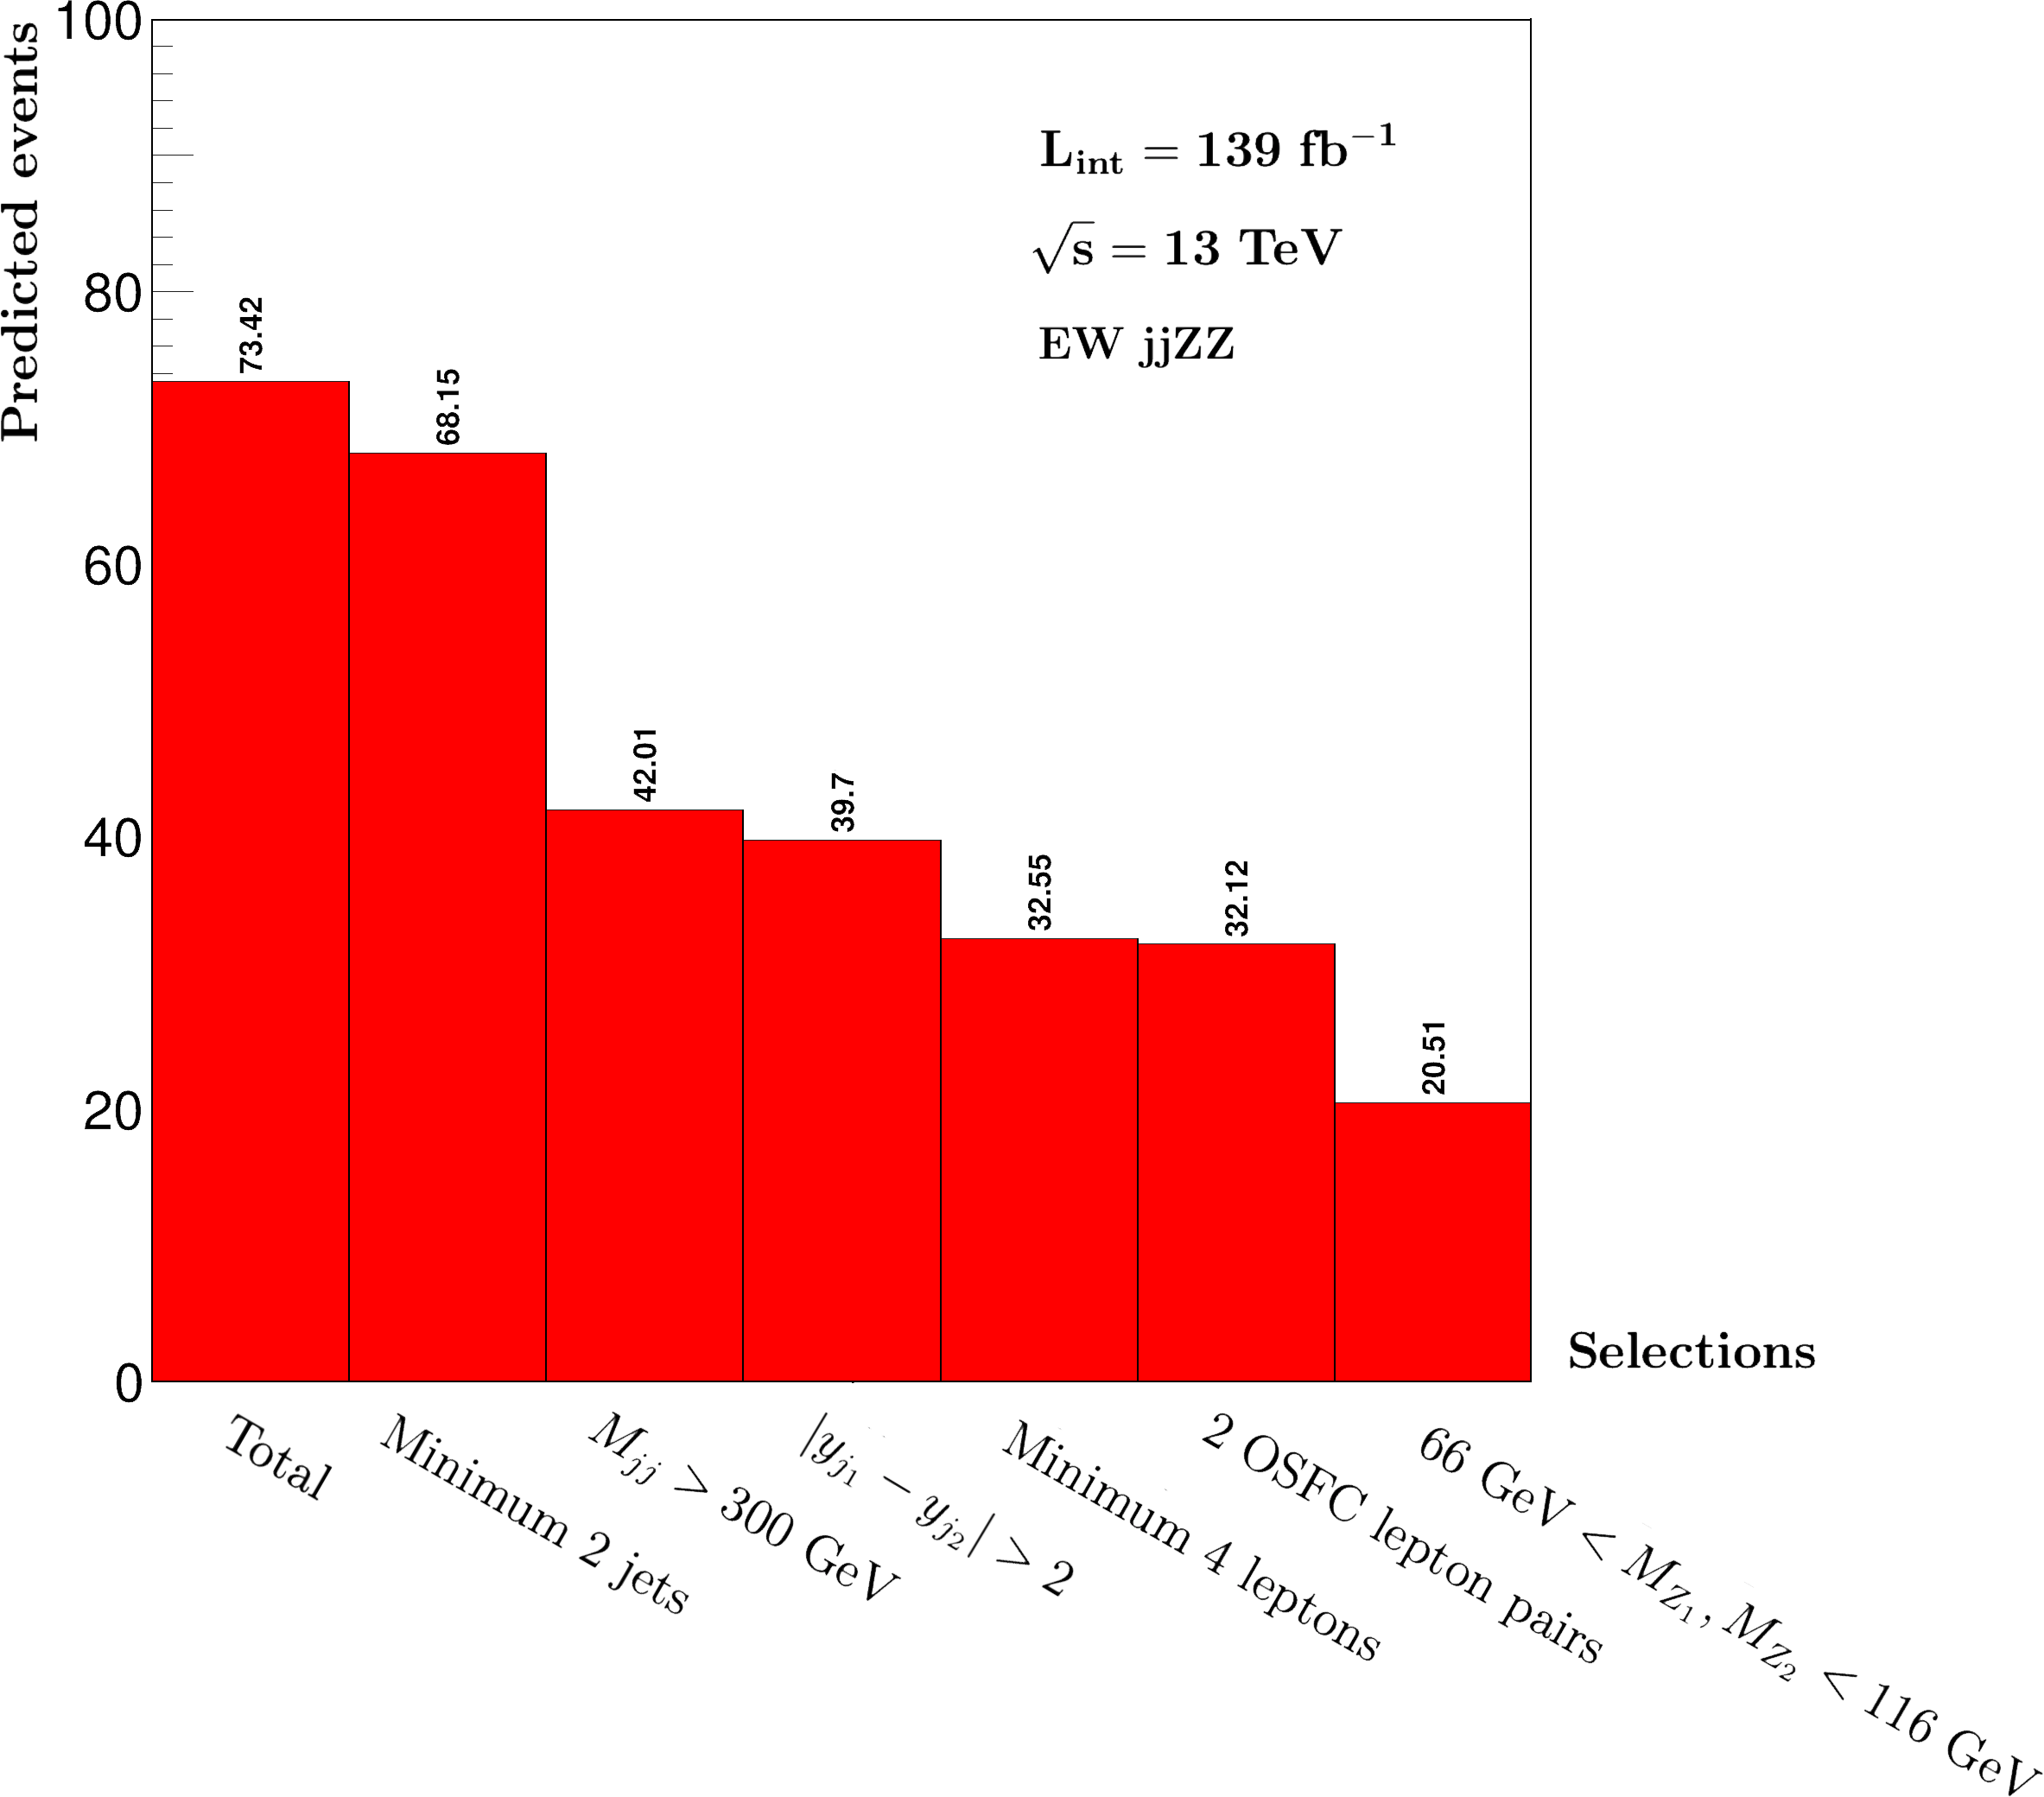
\includegraphics[scale=0.15]{cutflow_stack.png}
            \caption{Cutflow diagram of the predicted $EW\ jjZZ$ event number after selection cuts. Uncertainty was omitted and numbers 
            after the decimal point were preserved.}
            \end{centering}
        \end{figure}
    \section{Background and uncertainty}
        \par The $jjZZ4l$ channel contain 3 major processes, namely $EW ZZ4l$, $S qqZZ4l$ and $S ggZZ4l$,
        background process come mainly form process involve top quark, other contributions are small.
        In this stage of measurement, all processes were modeled using the simulation events, the $VH$, triboson,
        $WZ$ process and processes with top quark in leading order can produce same or similar final state
        with signal process, if leptons or jets was misidentified, they can potentially fake $jjZZ4l$ process, from now on 
        denote ``Other'' process. 
        there are potential to usr data driven methods to constrain the background in future analysis.
        \par With only detector level selection, the predicted distribution of 4-lepton imvarient mass ($M_{4l}$) is shown in Figure 4, 
        in which we can clearly see the single Z boson resonance around 91 GeV dominated by $S qq4l$ process, 
        Higgs resonance around 125 GeV dominated by $S ggH4l$ process, and the ``shoulder'' of Z boson pair mass starting from about 182 GeV.

        \begin{figure}[ht]
            \begin{centering}
            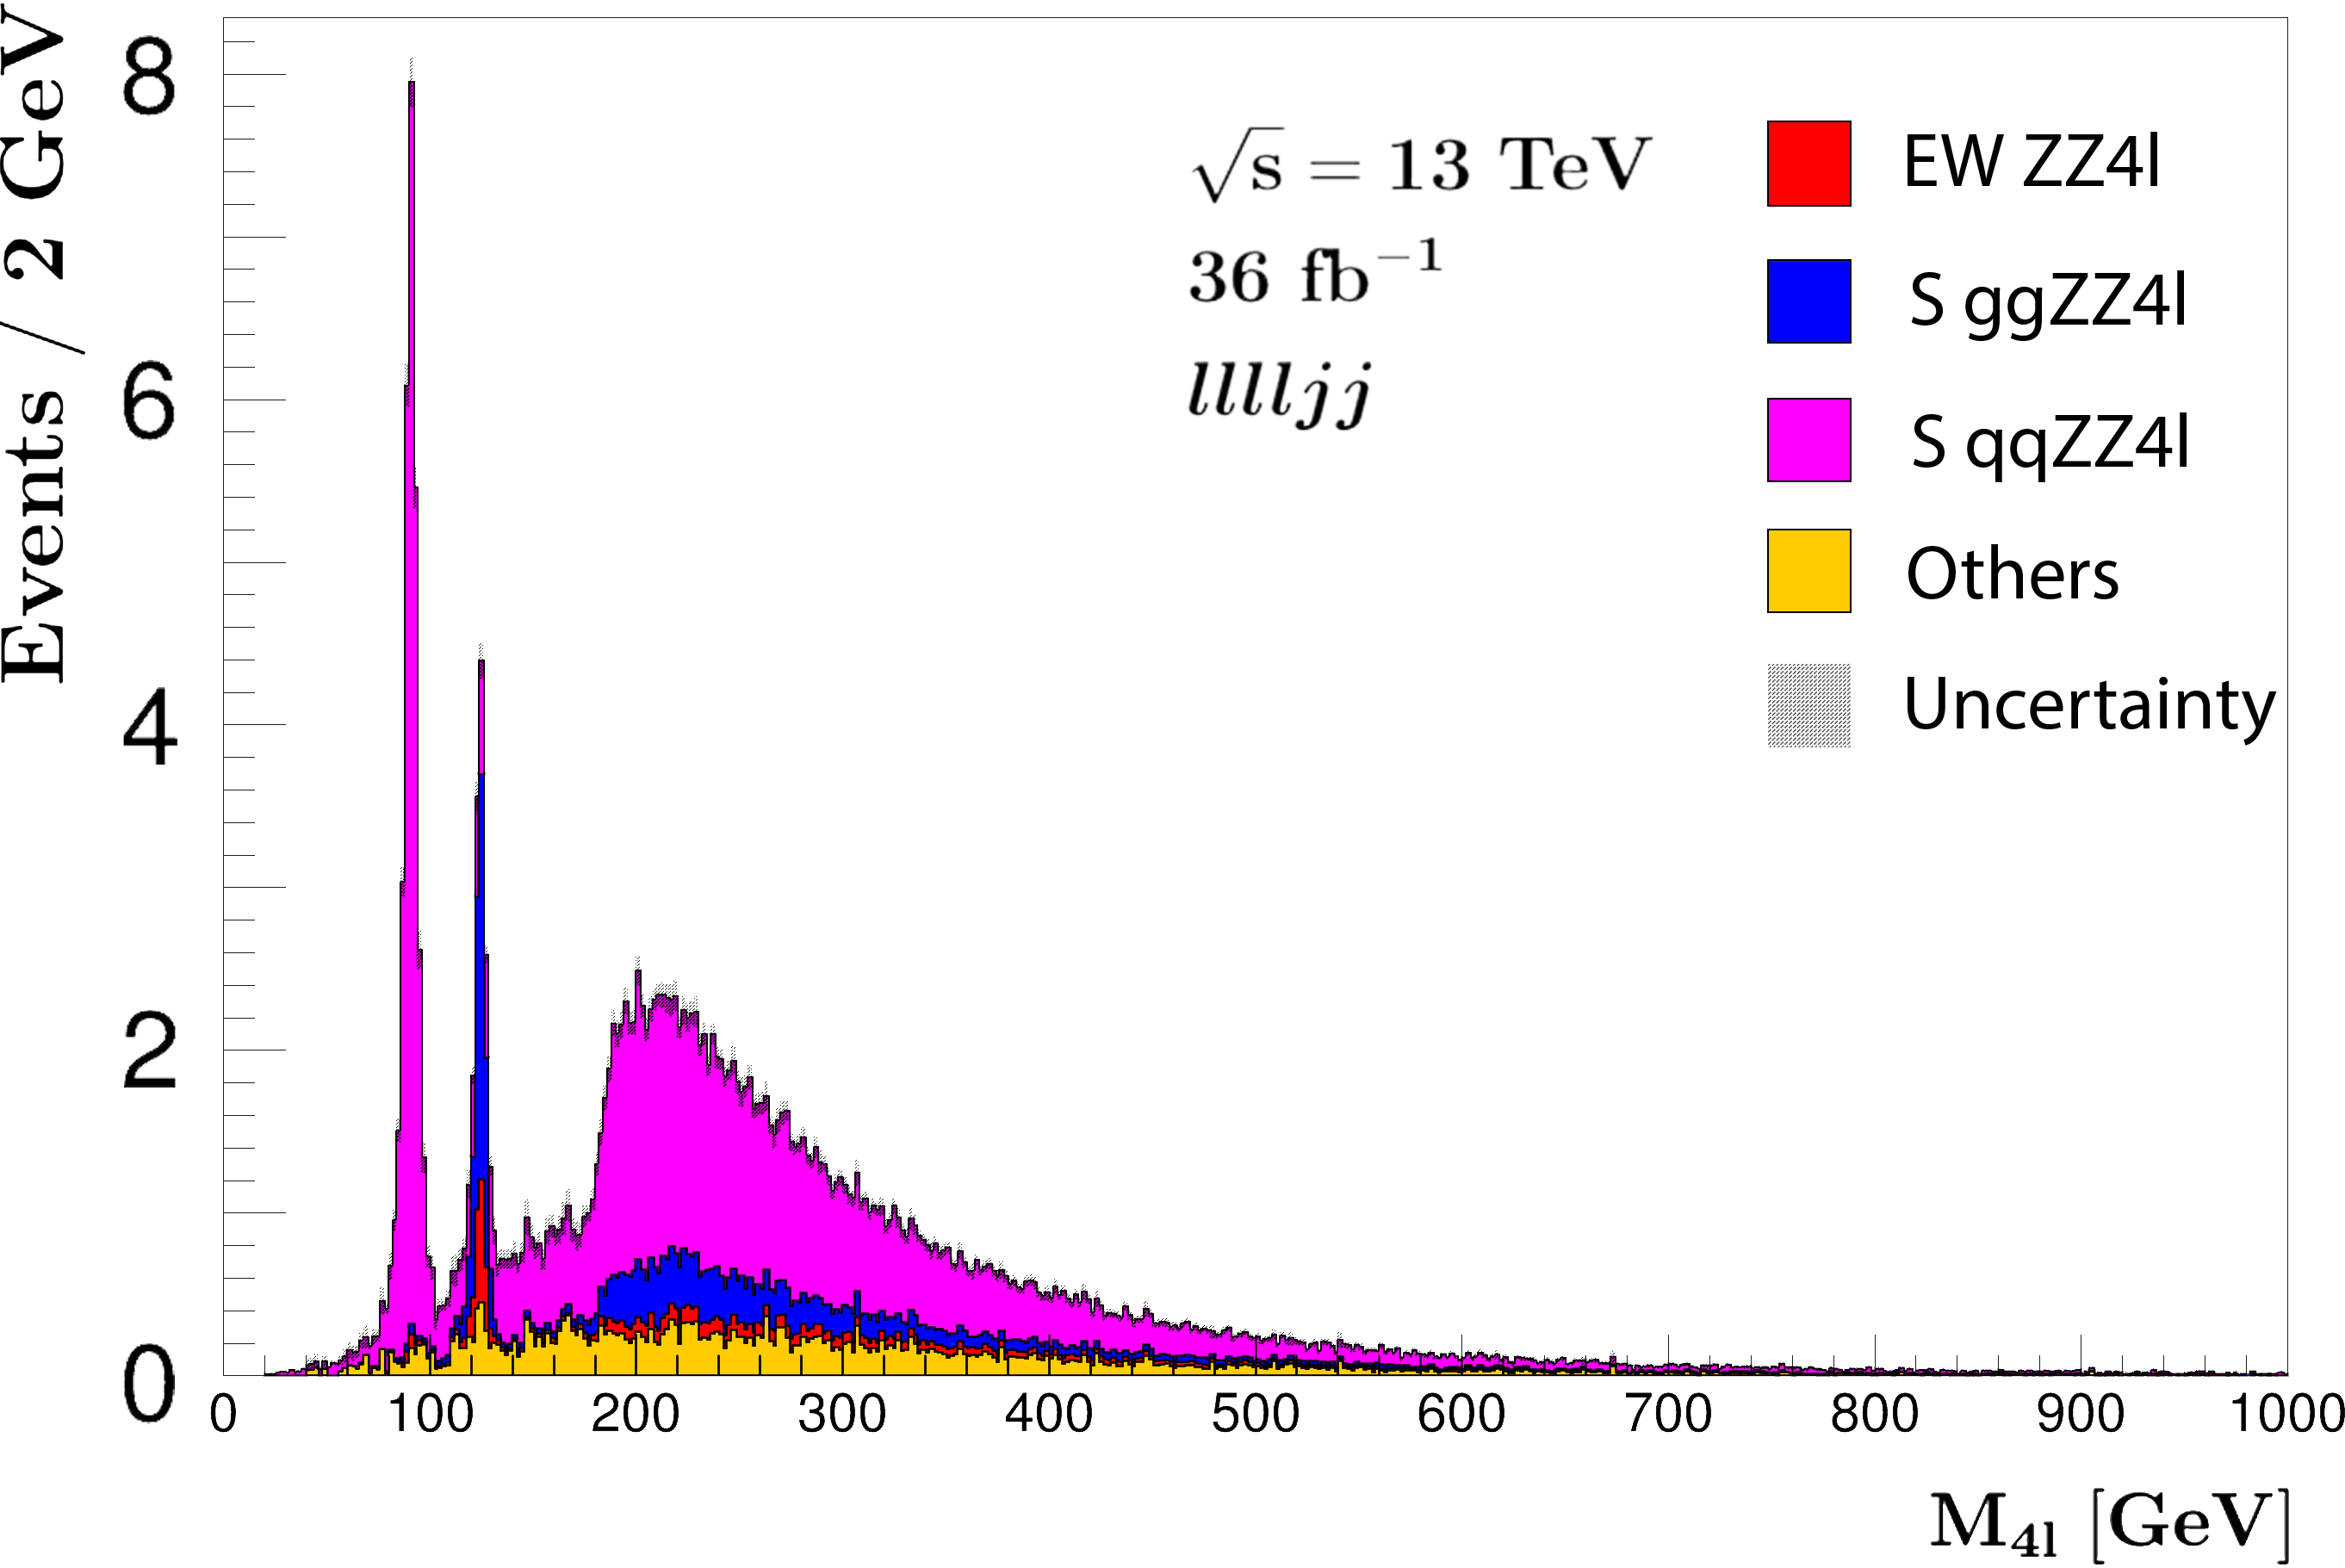
\includegraphics[scale=0.15]{ps/det_llll_m_stack.png}
            \caption{Predicted $M_{4l}$ distribution, with main resonance features shown clearly.}
            \end{centering}
        \end{figure}
        \par 
        

    \section{detector effect removal}
        why unfold and how, limitations; and its results. 
    \section{Discussion}
        what further work can be done. (preunfold, setlimits, more data, CP violation) 
    \section{Conclusion}

    \bibliographystyle{plain}
    \bibliography{bibli.bib}
    
\end{document}